\documentclass[11pt]{article}
\newcommand{\oa}{\overline{a}}
\newcommand{\ob}{\overline{b}}
\newcommand{\oc}{\overline{c}}
\newcommand{\oi}{\overline{i}}

\newcommand{\integermodn}[1][n]{\Z/#1\Z}
\newcommand{\integermodnmul}[1][n]{(\Z/#1\Z)^{\times}}
\newcommand{\order}[1]{\left|#1\right|}
\newcommand{\modb}[1]{\left(mod \;\; #1 \right)}
\newcommand{\aut}[1]{Aut\left(#1\right)}
\newcommand{\actson}{\ensuremath{\curvearrowright}}

\newcommand{\heading}[1]{(#1)}
\newcommand{\bheading}[1]{\textbf{(#1)}}

% arg1=pdfurl arg2=pagenum arg3=text
\usepackage{url}
\usepackage{hyperref}
\hypersetup{colorlinks=true, linktoc=all, linkcolor=blue}
\newcommand{\linkbook}[3][../../abstract_algebra_dummit_and_foote.pdf]{
    \noindent\href[page=#2]{#1}{\urlstyle{rm}{#3}}
}

\usepackage[a4paper, total={6in, 8in}, margin=0.5in]{geometry}


\graphicspath{{../assets/}}

\begin{document}

\linkbook{7}{table of contents}
\linkbook{21}{flow chart}
\tableofcontents

\newpage
\begin{center}
    Basics
\end{center}

\begin{enumerate}
    \item \bheading{Taylor Expansion} Given $f \in C^{\infty}(\R)$, the Taylor expansion of $f$ at $a$ is given by 
    \begin{align*}
        T(a)
        &= \sum_{n=0}^{\infty} \frac{f^{(n)}(a)}{n!} (x-a)^n \\
        &= f(a) + \frac{f'(a)}{1!}(x-a) + \frac{f''(a)}{2!} (x-a)^2 + \cdots
    \end{align*}
    \item \bheading{Taylor's Theorem} Let $k\geq 1$ and function $f:\R\to\R$ be $k$ times differentiable at a point $a\in \R$, then exists $h_k:\R\to\R$ such that 
    \[
        f(x)
        = \sum_{n=0}^{k} \frac{f^{(n)}(a)}{n!} (x-a)^n + h_k(x) (x-a)^k
    \]
    and $\lim_{x\to a} h_k(x) = 0$, i.e. the reminder term $R_k(x) = f(x) - P_k(x)$ is asymptotically trivial. If $f$ is $k+1$ times differentiable on the open interval and $f^k$ continous on the closed interval $[a,x]$, then the Lagrange remind is given by 
    \[
        R_k(x) = \frac{f^{k+1}(\zeta)}{(k+1)!} (x-a)^{k+1}
    \]
    for soem $\zeta \in [a,x]$ by the mean value theorem
    \item \bheading{Taylor's Theorem for multivariable function} If $f:\R^n\to \R$ are $k$ times differentiable function at point $\ba\in\R^n$ then exists $h_{\alpha}: \R^n \to \R$ such that 
    \[
        f(\bx) = \sum_{|\alpha| \leq k} \frac{D^{\alpha}f(\ba)}{\alpha!}(\bx-\ba)^{\alpha} + \sum_{|\alpha|=k} h_{\alpha}(\bx) (\bx - \ba)^{\alpha}
        \quad \quad \lim_{\bx \to \ba} h_{\alpha}(\bx) = 0
    \]
    where 
    \[
        |\alpha| = \alpha_1 + \cdots + \alpha_n
        \quad \quad 
        \alpha! = \alpha_1!\cdots \alpha_n!
        \quad \quad
        \bx^{\alpha} = x_1^{\alpha_1} \cdots x_n^{\alpha_n}    
        \quad \quad 
        D^{\alpha}f = \frac{\partial^{|\alpha|} f}{\partial x_1^{\alpha_1} \cdots x_n^{\alpha_n}}
    \]
    \item \bheading{$\sO$ notation} $f(x) = \sO(g(x))$   describes asymptotic behavior of function $f$
    \begin{enumerate}
        \item \heading{as $x\to \infty$} if there exists $M\geq 0$ and $x_0\in\R$ such that $|f(x)| \leq M g(x)$ for all $x>x_0$. 
        \item \heading{as $x\to a$} if there exists $M\geq 0$ and $\delta \in\R$ such that $|f(x)| \leq M g(x)$ when $0 < |x-a| < \delta$. Alternatively we can say 
        \[
            \lim_{x\to a} \sup \abs{\frac{f(x)}{g(x)}} < \infty
        \]
    \end{enumerate}
    \item \bheading{binomial theorem} 
    \[
        (x+y)^n = \sum_{k=0}^n  \binom{n}{k} x^{n-k} y^k
    \]
    \item \bheading{power series expansions}
    \begin{align*}
        \frac{1}{1-x} 
            &= \sum_{n=0}^{\infty} x^n = 1+x+x^2+x^3+\cdots \\
        e^x 
            &= \sum_{n=0}^{\infty} \frac{x^n}{n!} = 1+x+\frac{x^2}{2}+\frac{x^3}{3!}+\cdots \\
        (1+x)^{\alpha}
            &= \sum_{k=0}^{\infty} \binom{\alpha}{k} x^k \\
        \ln(1+x)
            &= \sum_{n=1}^{\infty} (-1)^{n+1} \frac{x^n}{n} = x - \frac{x^2}{2} + \frac{x^3}{3} \tag{convergent if $|x|<1$} \\
        \ln(1-x)
            &= \sum_{n=1}^{\infty} \frac{x^n}{n} = x + \frac{x^2}{2} + \frac{x^3}{3} \tag{convergent if $|x|<1$} \\
        \sin x
            &= \sum_{n=0}^{\infty} \frac{(-1)^n}{(2n+1)!} x^{2n+1}
            = x - \frac{1}{3!} x^3 + \frac{1}{5!} x^5 + \cdots \\
        \sin^2 x 
            &= \sum_{n=1}^{\infty} \frac{(-1)^{n+1} 2^{2n-1} x^{2n}}{(2n)!}
            = \frac{2 x^2}{2!} - \frac{8x^4}{4!} + \frac{32 x^6}{6!} + 
    \end{align*}
    \item \bheading{trigonometric identities}
    \begin{align*}
        \sin (\theta + \phi) 
            &= \sin(\theta)\cos(\phi) + \sin(\phi)\sin(\theta) \\
        \sin (\theta + \phi) + \sin (\theta - \phi)
            &= 2\sin (\theta) \cos(\phi) \\
        1 - \cos(\theta) = 2\sin^2 \p{\frac{\theta}{2}}
    \end{align*}
\end{enumerate}


\section{\linkbook{25}{Euler's Method and Beyond}}

\subsection{\linkbook{25}{Ordinary differential equations and Lipschitz condition}}


\begin{enumerate}
    \item \bheading{Goal} Approximate solution to 
    \[
        \by' = \bf ( t, \by)
        \quad \text{with initial condition} \quad 
        \by ( t_0 ) = \by_0    
    \]
    where $t > t_0$ and $\bf: [t_0, \infty) \times \R^d \to \R^d$ is a sufficiently well behaved function
    \item \bheading{Lipschitz condition} Given $\bf$ and norm $\norm{\cdot}$, the Lipschitz condition is defined by 
    \[
        \norm{
            \bf(t, \bx) - \bf(t, \by)
        } \leq \lambda \norm{\bx - \by}
        \quad \quad
        \text{for all}
        \quad \bx, \by \in \R^d \;,\; t> t_0
    \]
    where $\lambda \in \R$ is called Lipschitz constant. 
    \item \bheading{Picard Lindelof theorem} Consider initial value problem 
    \[
        y'(t) = f(t, y(t))
        \quad
        y(t_0) = y_0
    \]
    If $f$ is uniformly Lipschitz continous in $y$ and continous in $t$, then for some $\epsilon > 0$, there exists unique solution $y(t)$ to the initial value problem on the interval $[t_0 - \epsilon, t_0 + \epsilon]$ 
    \item \bheading{Analytic function} A function $\bf$ is an analytic function if it is a function that is locally given by a convergent power series, i.e. an infinitely differentiable function such that at any point $(t,\by_0) \in [0, \infty)\times \R^d$ in its domain, the Taylor series converges to $\bf(\bx)$ for $\bx$ in a neighborhood of $(t,\by_0)$.
    \begin{enumerate}
        \item \heading{example} polynomial, exponential, trigonometric, logarithm, power function
        \item \heading{note} if $\bf$ is analytic, solution $\by$ to the initial value problem is also analytic
    \end{enumerate}
\end{enumerate}


\subsection{\linkbook{26}{Euler's method}}

\begin{definition*}
    \bheading{Euler's Method} Given initial value problem $\by' = \bf(t, \by)$ for $t\geq t_0$ and initial value $\by(t_0) = \by_0$. If we assume $\by'(t) = \bf(t, \by(t)) \approx \bf(t_0, \by(t_0))$ for $t\in [t_0,t_0+h)$ (i.e. deriviative in $[t_n, t_{n+1}]$ is approximated by value of derivative at $t_n$) for some sufficiently small time step $h>0$, we can approximate the value of $\by(t)$ by
    \begin{align*}
        \by(t) 
        &= \by(t_0) + \int_{t_0}^t \bf(\tau, \by(\tau)) d\tau  \\
        &\approx \by_0 + (t-t_0) \bf(t_0, \by_0)
    \end{align*}
    Given a sequence of times $(t_n)_{n\in\N} = \p{t_0, t_0+h,\cdots}$ we have numerical approximation $(\by_n)_{n\in\N}$ by 
    \[
        \by_{n+1} = \by_n + h\bf(t_n, \by_n)
    \]
    \begin{enumerate}
        \item \heading{intuition} euler's method is a time-stepping numerical method that covers interval by an equidistant grid and produe numerical solution at the grid points. we can show that euler's method is convergent, i.e. as $h\to 0$, grid is refined, the numerical solution tends to exact solution
    \end{enumerate}
\end{definition*}

\begin{definition*}
    \bheading{convergent method} Given a time-stepping numerical method on a compact inteval $[t_0, t_0+t^*]$, we can compute numerical solutions dependent upon $h$
    \[
        \by_n = \by_{n,h}
        \quad \text{for}
        \quad n = 0,1,\cdots,\lfloor t^*/h\rfloor    
    \]
    A method is said to be convergent if for every ODE with Lipschitz function $\bf$, the numerical solution tends to the true solution as the grid becomes increasingly fine. More rigorously, if every ODE with Lipschitz function $\by$ and for every $t^*>0$, then following holds 
    \[
        \lim_{h\to 0^+} \max_{n=0,1,\cdots,\lfloor t*/h\rfloor    } \norm{\by_{n,h} - \by(t_n)} = 0
    \]
\end{definition*}

\begin{theorem*}
    \bheading{Euler's method is convergent} 
    \begin{proof}
        Assume $\bf$ and therefore also $\by$ is analytic, i.e. convergent Taylor expansion. Let $\be_{n,h} = \by_{n,h} - \by(t_n)$ be the numerical error. Show $\lim_{h\to 0^+} \max_n \norm{\be_{n,h}} = 0$. By Taylor's theorem 
        \[
            \by(t_{n+1})
            = \by(t_n) + h\by'(t_n) + \sO(h^2)
            = \by(t_n) + h\bf(t_n,\by(t_n)) + \sO(h^2)
        \]
        given $\by$ continously differentiable, $\sO(h^2)$ can be bounded uniformly for all $h>0$ by a term $ch^2$ for some $c>0$. Subtract previous from iterative formula of euler's method 
        \[
            \be_{n+1,h} = 
            \be_{n,h} + h\p{
                \bf(t_n, \by(t_n) + \be_{n,h}) - \bf(t_m, \by(t_n))
            } + \sO(h^2)
        \]
        By triangle inequality and Lipschitz condition 
        \begin{align*}
            \norm{\be_{n+1, h}}
            &\leq \norm{\be_{n,h}} + h\norm{\bf(t_n, \by(t_n) + \be_{n,h}) - \bf(t_n, \by(t_n))} + ch^2 \\
            &\leq (1+h\lambda) \norm{\be_{n,h}} + ch^2
        \end{align*}
        for $n=0,1,\cdots,\lfloor t^*/h \rfloor - 1$. By induction on $n$, we can show $\norm{\be_{n,h}} \leq \frac{c}{\lambda} h \p{(1+h\lambda)^n - 1}$. Since $1+h\lambda < e^{h\lambda}$ we have $(1+h\lambda)^n < e^{nh\lambda} < e^{\lfloor t*/h\rfloor h\lambda} \leq e^{t^* \lambda}$. Therefore 
        \[
            \norm{\be_{n,h}}   \leq \frac{c}{\lambda} (e^{t^*\lambda} - 1)h
        \]
        for $n=0,1,\cdots,\lfloor t*/h\rfloor$. This is an upper bound on the error that is independent of $h$, hence $\lim_{h\to 0} \norm{\be_{n,h}} = 0$. from which we can infer that error decays globally as $\sO(h)$
    \end{proof}
\end{theorem*}

\begin{definition*}
    \bheading{order $p$ method} Given arbitrary time-stepping method 
    \[
        \by_{n+1} = \bsY_n (\bf, h. \by_0, \by_1, \cdots, \by_n) \quad \quad n = 0,1,\cdots   
    \]
    for initial value problem, it is of order $p$ if 
    \[
        \by(t_{n+1}) - \bsY_n (\bf, h, \by(t_0), \by(t_1), \cdots, \by(t_n)) = \sO(h^{p+1})
    \]
    for every analytic $\bf$ and $n=0,1,\cdots$. Intuitively, a method is of order $p$ if it recovers exactly every polynomial oslution of degrees $p$ or less.
    \begin{enumerate}
        \item \heading{intuition} order of a method gives information about local behavior, i.e. advancing from $t_n$ to $t_{n+1}$ where $h>0$ is sufficiently small, we are incurring an error of $\sO(h^{p+1})$. Generally want the the global (convergence) behavior of the method instead.
        \item \bheading{fact} euler's method is order 1
        \begin{proof}
            Euler's method can be written as $\by_{n+1} - \p{\by_n + h\bf(t_n, \by_n)} = 0$. Replace $\by_k$ by $\by(t_k)$ and expand terms of Taylor series about $t_n$ we have 
            \[
                \by(t_{n+1}) - \p{\by(t_n) + h\bf(t_n, \by(t_n))}
                 = \p{
                     \by(t_n) + h\by'(t_n) + \sO(h^2)
                 } - \p{
                     \by(t_n) + h\by'(t_n)
                 } = \sO(h^2)
            \]
        \end{proof}
    \end{enumerate}
\end{definition*}



\subsection{\linkbook{30}{The trapezoidal rule}}


\begin{definition*}
    \bheading{Trapezoidal Rule} Instead of approximating derivative by a constant in $[t_n, t_{n+1}]$, namely by its value at $t_n$, the trapezoidal rule approximates the value of the derivate by average of values at the endpoints. We can approximate solution $\by(t)$ by 
    \begin{align*}
        \by(t) 
        &= \by(t_n) + \int_{t_n}^t \bf(\tau, \bf(\tau)) d\tau \\
        &\approx \by(t_n) + \frac{1}{2} (t-t_n) \p{\bf(t_n, \by(t_n)) + \bf(t, \by(t))}
    \end{align*}
    Given a sequence of times $(t_n)_{n\in\N} = \p{t_0, t_0+h,\cdots}$ we have numerical approximation $(\by_n)_{n\in\N}$ by 
    \[
        \by_{n+1} = \by_n + \frac{1}{2} h \p{
            \bf(t_n, \by_n) + \bf(t_{n+1}, \by_{n+1})
        }
    \]
    \begin{enumerate}
        \item \bheading{theorem} order of trapezoidal rule is 2
        \begin{proof}
            Compute by performing Taylor expansion on $\by(t_{n+1})$ and $\by'(t_{n+1})$ about $t_n$
            \[
                \by(t_{n+1}) - \pc{
                    \by(t_n) + \frac{1}{2}h \pc{
                        \bf(t_n, \by(t_n)) + \bf(t_{n+1}, \by(t_{n+1}))
                    }
                } = \sO(h^3)
            \]
        \end{proof}
        \item \bheading{theorem} trapezoidal rule is convergent
        \begin{proof}
            Detail of proof \linkbook{31}{here}. We can show error is bounded by 
            \[
                \norm{\be_{n,h}}\leq \frac{ch^2}{\lambda} exp \p{
                    \frac{t^* \lambda}{1 - \frac{1}{2}h\lambda}
                }
            \]
            from which we can infer that error decays globally as $\sO(h^2)$
        \end{proof}
        \item \heading{note} euler's method is explicit, since we can compute $\by_{n+1}$ with a few arithmetic operations by computing $\bf$, a function of a known $\by_n$. Trapezoidal rule is implicit, i.e. finding $\by_{n+1}$ is not trivial and $\bf$ is a function of both $\by_n$ and $\by_{n+1}$. We might need to solve a nonlinear equation of $\by_{n+1}$
        \[
            \by_{n+1} - \frac{1}{2}h \bf(t_{n+1}, \by_{n+1}) = \bv
        \]
        where $\bv = \by_n + \textstyle \frac{1}{2} h \bf(t_n, \by_n)$ can be evaluated easily from assumptions.
    \end{enumerate}
\end{definition*}



\subsection{\linkbook{35}{The theta method}}

\begin{definition*}
    \bheading{theta method} is a generalization of Euler's method ($\theta=1$) and the trapezoidal rule ($\theta = 1/2$), whereby the derivates are assumed to be piecewise constant and provided by a linear combination of derivatives at the endpoints of each interval. The numerical approximates are,
    \[
        \by_{n+1} = \by_n + h\p{
            \theta \bf(t_n, \by_n) + (1-\theta) \bf(t_{n+1}, \by_{n+1})
        }
        \quad \quad n = 0,1,\cdots
    \]
    for some fixed $\theta \in [0,1]$
    \begin{enumerate}
        \item \heading{fact} theta method is explicit for $\theta=1$ and implicit otherwise
        \item \bheading{theorem} theta method is of order 2 for $\theta=1/2$ and order 1 otherwise.
        \item \bheading{theorem} theta method is convergent for every $\theta \in [0,1]$
    \end{enumerate}
\end{definition*}



\section{\linkbook{41}{Multistep Method}}



\section{\linkbook{161}{8 Finite Differences Schemes}}

\subsection{\linkbook{161}{8.1 Finite differences}}


\begin{enumerate}
    \item \bheading{Finite difference operators} Given real sequences $\bz = \pc{z_k}_{k\in\Z} = z(kh)$ for $k\in\Z$ as discrete sampling of a function $z$ for some $h>0$. Let $x_k = kh$. We can define finite difference operators mapping the space $\R^{\Z}$ of all such sequences to itself.
    \begin{align*}
        (\shift \bz)_k 
            &= z_{k+1} \tag{shift} \\
        (\forw \bz)_k  
            &= z_{k+1} - z_k \tag{forward difference} \\
        (\back \bz)_k 
            &= z_k - z_{k-1} \tag{backward difference} \\
        (\cent \bz)_k 
            &= z_{k+\frac{1}{2}} - z_{k - \frac{1}{2}} \tag{central difference} \\
        (\avg \bz)_k 
            &= \textstyle\frac{1}{2} (z_{k-\frac{1}{2}} + z_{k+\frac{1}{2}}) \tag{averaging}
    \end{align*}
    Finite difference operators are composed under function composition.
    \begin{enumerate}
        \item \bheading{fact} $\sT \in \pc{\shift, \forw, \back, \cent, \avg, \diff}$ are linear operators
        \[
            \sT(a\bw + b\bz) = a\sT\bw + b\sT\bz
            \quad \text{ for } \quad
            \bw,\bz\in\R^{\Z}\;,\;\; a,b\in\R    
        \]
        \item \bheading{convention} $\sT z_k$ stands for $(\sT \bz)_k$
    \end{enumerate} 
    \item \bheading{Differential operator} The goal is to approximate derivatives $\diff$ by expresing it with a linear combination of values along the grid.
    \begin{align*}
        (\diff\bz)_k &= z'(kh) \tag{differential}
    \end{align*}
    \item \bheading{Functions of operators} Finite difference operators are functions of $h$. Given an analytic function as Taylor series, $g(x) = \textstyle\sum_{j=0}^{\infty} a_j x^j$, we can expand $g$ about $\pc{\shift-\id, \avg - \id, \forw, \back, \cent, h\diff}$,
    \[
        g(\forw)\bz = \p{
            \sum_{j=0}^{\infty} a_j \forw^j
        } \bz = 
        \sum_{j=0}^{\infty} a_j (\forw^j \bz)
    \]
    \item \bheading{Asymptotics of operators}
    \[
        \pc{\shift-\id, \avg - \id, \forw, \back, \cent, h\diff} \overset{h\to 0+}{\longrightarrow} O
    \]
    \begin{enumerate}
        \item \bheading{example} 
        \[
            \forw z_k = z_{k+1} - z_k =  z(x_k + h) - z(x_k) = hz'(\eta_k) = \sO(h)
        \]
        by some $\eta_k \in [x_k, x_{k+1}]$ by mean value theorem
    \end{enumerate}
    \item \bheading{Operator $\shift^{1/2}$}
    \[
        (\shift^{1/2} \bz)_k = z((k+\frac{1}{2})h)
    \]
    by defining it with a power series expansion of $g(x) = \sqrt{1+x}$
    \[
        \shift^{1/2} = (\id + (\shift - \id))^{1/2} = \id + \sum_{j=0}^{\infty} \frac{ (-1)^{j-1} }{ 2^{2j - 1} } \frac{(2j - 2)!}{(j-1)!j!}  (\shift - \id)^j
    \]
    \item \bheading{Operator commutativity} Idea is all operator can be expressed w.r.t. $\shift$
    \begin{align*}
        \forw 
            &= \shift - \id \\
        \back
            &= \id - \shift^{-1} \\ 
        \cent
            &= \shift^{1/2} - \shift^{-1/2} \\
        \avg
            &= \frac{1}{2} (\shift^{1/2} + \shift^{-1/2}) \\
        \id
            &= \shift^0 \\
        h\diff
            &= \ln \shift
    \end{align*}
    \begin{proof}
        Rest are trivial. To show $h\diff = \ln\shift$, note 
        \[
            \shift z(x) = z(x+h) = 
            \sum_{i=0}^{\infty} \frac{h^i}{i!} \frac{d^i z(x)}{dx^i}
            = \pb{
                \sum_{i=0}^{\infty} \frac{1}{i!} (h\diff)^i
            } z(x)
            = e^{h\diff} z(x)
        \]
    \end{proof}
    \item \bheading{rewrite $\diff$ in terms of $\forw, \back, \cent$} 
    \begin{align*}
        h\diff
            &= \ln \p{\id + \forw} \\
        h\diff
            &= -\ln \p{\id - \back} \\
        h\diff
            &= 2\ln \p{\frac{1}{2}\cent + \sqrt{\id + \frac{1}{4}\cent^2}}
    \end{align*}
    \begin{proof}
        From previous, $\shift = \id + \forw = \p{\id - \back}^{-1}$. For the last expression, consider
        \begin{align*}
            \cent &= \shift^{1/2} - \shift^{-1/2} \\
            \shift^{1/2} \cent &= \shift - \id \\
            (\shift^{1/2})^2 - \shift^{1/2}\cent - \id &= 0\\
            \shift^{1/2} &= \frac{1}{2} \cent \pm \sqrt{\id + \frac{1}{4}\cent^2} \tag{$+$ is correct}\\
            \shift &= \p{
                \frac{1}{2}\cent + \sqrt{\id + \frac{1}{4}\cent^2}
            }^2
        \end{align*}
    \end{proof}
    \item \bheading{approximate $\diff$ and its powers} To approximate $\diff$ with $\forw$, we can expand $\ln\p{\id + \forw}$ by power series expansion of $\ln(1+x) = \textstyle\sum_{i=1}^{\infty} (-1)^{n+1} \frac{x^i}{i!}$ 
    \begin{align*}
        \diff 
        &= \frac{1}{h} \ln\p{\id + \forw}
        = \frac{1}{h} \pb{
            \forw - \frac{1}{2} \forw^2 + \frac{1}{3} \forw^3 + \sO(\forw^4)
        } \\
        &= \frac{1}{h} \p{
            \forw - \frac{1}{2} \forw^2 + \frac{1}{3} \forw^3
        } + \sO(h^3) \quad \quad h\to 0
    \end{align*}
    where $\forw = \sO(h)$ as $h\to 0$ shown perviously. Use binomial theorem on $\diff$ repeatedly and collect terms to $\sO(h^3)$, 
    \[
        \diff^s = \frac{1}{h^s}\pb{
            \forw^s - \frac{1}{2} s \forw^{s+1} + \frac{1}{24} s(3s + 5) \forw^{s+2}
        } + \sO(h^3)  \quad \quad h\to 0
    \]
    Inuititively, we can approximate $\diff^s z_k = d^s z(kh)/ dx^s$ up to $\sO(h^3)$ with $s+3$ grid points in the positive direction, i.e. $z_k, z_{k+1}, \cdots, z_{k+s+2}$. Similarly we can express $\diff$ in terms of grid points to the left with $\back$.
    \[
        \diff^s = \frac{(-1)^s}{h^s} \p{\ln\p{\id - \back}}^s
        = \frac{1}{h^s} \pb{
            \back^s + \frac{1}{2} s \back^{s+1} + \frac{1}{24} s(3s + 5) \back^{s+2}
        } + \sO(h^3)  \quad \quad h\to 0
    \]
    Similarly we can express $\diff$ in terms of grid points on the left and right with $\cent$ operator. Note, only even powers of $\cent$ maps $\R^{\Z} \to \R^{\Z}$, i.e. onto grid points. ($\cent^2 z_k = z_{k+1} -2z_k + z_{k-1}$ and for any power to $2s$, $\cent^{2s} = \p{\cent^2}^{^s}$). We consider Maclaurin expansion of function $g(\xi) = \ln(\xi + \sqrt{1+\xi^2})$
    \[
        g(\xi) = 2 \sum_{j=0}^{\infty} \frac{(-1)^j}{2j + 1} \binom{2j}{j} \p{\frac{1}{2} \xi}^{2j+1}    
    \]
    Let $\xi = \textstyle\frac{1}{2} \cent$, we have power series expansion of $\diff$ in terms of $\cent$
    \[
        \diff = \frac{2}{h} g(\frac{1}{2} \cent)
        = \frac{4}{h} \sum_{j=0}^{\infty} \frac{(-1)^j}{2j+1} \binom{2j}{j} \p{\frac{1}{4} \cent}^{2j+1}
    \]
    However powers of $\cent$ are all odd, we raise power to $2s$ to keep output of operator on the grid
    \[
        \diff^{2s} = \frac{1}{h^{2s}}     \pb{
            \p{\cent^2}^s - \frac{s}{12} \p{\cent^2}^{s+1} + \frac{s(11+5s)}{1440} \p{\cent^2}^{s+2}
        } + \sO(h^6)
        \quad \quad  h\to 0
    \]
    approximates $\diff$ up to $\sO(h^6)$
    \item \bheading{comparing $\forw$ and $\cent$ for approximating $\diff$} To attain $\sO(h^{2p})$ error, $\forw$ requires $2s+2p$ grid points and $\cent$ requires $2s+2p-1$ grid points. However $\forw$ would have a smaller error constant. (exercise 8.3)
    \item \bheading{express $\avg$ in terms of $\cent$}
    \[
        \avg = \p{\id + \frac{1}{4}\cent^2}^{1/2}    
    \]
    \begin{proof}
    \begin{align*}
        \avg &= \frac{1}{2} \p{\shift^{1/2} + \shift^{-1/2}}
        \quad &\longrightarrow \quad
        4\avg^2 &= \shift + 2\id + \shift^{-1} \\
        \cent &= \shift^{1/2} - \shift^{-1/2}
        \quad &\longrightarrow \quad
        \cent^2 &= \shift - 2\id + \shift^{-1}
    \end{align*}
    Therefore $4\avg - \cent^2 = 4\id$ and result follows
    \end{proof}
    \item \bheading{approximate odd derivatives with $\avg$ with central difference} 
    \[
        \diff = \frac{1}{h} \p{\avg\cent} \pb{
            \sum_{j=0}^{\infty} (-1)^j \binom{2j}{j} \p{\frac{1}{16}\cent^2}^j
        }\pb{
            \sum_{i=0}^{\infty} \frac{(-1)^i}{2i + 1} \binom{2i}{i} \p{\frac{1}{16}\cent^2}^i
        }
    \]
    which are constructed from even powers of $\cent$ and $\avg\cent$ which will make image of $\diff$ operator reside on the grid.
    \[
        \avg\cent z_k = \avg \p{z_{k+\frac{1}{2}} - z_{k - \frac{1}{2}}} = \frac{1}{2}\p{z_{k+1} - z_{k-1}}
    \]
    Raising powers of $\diff$ yield
    \[
        \diff^{2} = \frac{1}{h^2} (\avg\cent)^2 (\id - \frac{1}{3}\cent^2) + \sO(h^4)
    \]
    \item \bheading{practical use} instead of mixing difference operators, opt for finite difference grids. For finite grids, one-sided finite differences can be employed to evaluate $\diff$ near boundaries. 
\end{enumerate}


\subsection{\linkbook{169}{8.2 The five-point formula for $\nabla^2 u = f$}}


\begin{enumerate}
    \item \bheading{consistent} A method is consistent if the truncation error goes to 0 as step size goes to zero
    \item \bheading{order of consistency} of $\sO(\Dx^p)+\sO(\Dy^q)$ is $p$ in $x$ and $q$ in $y$.
    \item \bheading{theorem} If a method is consistent and stable, then it is convergent and order of convergence will be same as the order of consistency
\end{enumerate}


\begin{enumerate}
    \item \bheading{Poisson Equation} 
    \[
        \nabla^2 u = ( \frac{\partial^2}{\partial x^2} + \frac{\partial^2}{\partial y^2}) u = f \quad \quad (x,y)\in\Omega
    \]
    and $f=f(x,y)$ is continuous, domain $\Omega\subset \R^2$ is bounded, open, and connected and has a piecewise-smooth boundary. Assume \textit{Dirichlet condition}, i.e. 
    \[
        u(x,y) = \phi(x,y) \quad \quad (x,y)\in \partial \Omega    
    \]
    \item \bheading{Setup} Inscribe a grid that is axis-aligned with equal spacing of $\Delta x$ in both direction, i.e. pick $\Delta x>0$, $(x_0, y_0) \in \Omega$ and let $\Omega_{\Delta x}$ be 
    \[
        \Omega_{\Delta x} = \pc{
            x_0 + k\Delta x, y_0 + l \Delta x
        } \subset \closure{\Omega}
    \]
    Denote 
    \begin{align*}
        \bI_{\Dx} &= \pc{
            (k,l)\in\Z^2 \mid (x_0 + k\Dx, y_0 + l\Dx) \subset \closure{\Omega}
        } \\
        \bI_{\Dx}^{\circ} &= \pc{
            (k,l)\in\Z^2 \mid (x_0 + k\Dx, y_0 + l\Dx) \subset \Omega
        }
    \end{align*}
    and for every $(k,l) \in \bI_{\Dx}^{\circ}$, let $u_{k,l}$ be \textit{approximation} to the solution $u(x_0 + k\Dx, y_0 + l\Dx)$ of the Poisson equation at the relevant grid point. Note there is no need to approximate points in $\bI_{\Dx} \setminus \bI_{\Dx}^{\circ}$ since they lie on $\partial \Omega$ and their exact values given by $\phi$.
    \item \bheading{internal, near-boundary, boundary points} A point on the grid $(k,l) \in \sI_{\Dx}$ whereby $(k\pm 1,l)$ and $(k, l\pm 1)$ are in $\bI_{\Dx}$ is called \textit{internal point}. A point $(k,l) \in \sI_{\Dx}$ where we can no longer employ a finite difference scheme (and so requires a special approach) is called \textit{near-boundary points}. $(k,l) \in \partial \Omega$ are called \textit{boundary points}
    \item \bheading{Central difference approximation} given $u$ sufficiently smooth, we can approximate $\nabla^2$
    \[
        \nabla^2 = \frac{1}{(\Dx)^2} \p{\vD_{0,x}^2 + \vD_{0,y}^2} + \sO(\p{\Dx}^2)
        \quad \text{where} \quad
        \frac{\partial^2 u}{\partial x^2} = \frac{1}{\Dx^2} \vD_{0,x}^2 u_{k,l} + \sO((\Dx)^2)
    \]
    with central difference operators, i.e. $\vD_{0,x}, \vD_{0,y}$ along the x,y-axis.We can rewrite Poisson equation by the \textit{five point} finite difference scheme. For every internal grid point $(k,l)$, we have 
    \[
        \frac{1}{(\Dx)^2} (\vD_{0,x}^2 + \vD_{0, y}^2) u_{k,l} = f_{k,l}
    \]
    where $f_{k,l} = f(x_0 + k\Dx, y_0 + l\Dx)$. Expanding expression, we have
    \[
        u_{k-1,l} + u_{k+1, l} + u_{k, l-1} + u_{k, l+1} - 4u_{k,l} = (\Dx)^2 f_{k,l}    
    \]
    Intuitively, we have a linear combination of values of $u$ at grid point and at immediate horizontal and vertical neighbors of this point.
    \item \bheading{properties}
    \begin{enumerate}
        \item \bheading{truncation error} $\sO(\Dx^2) + \sO(\Dy^2)$ (computed by substituting exact solution $\tu_{i,j} = u(x_0+\Dx,y_0+\Dy)$ to finite difference formula in place of approximate values at grid points $u_{i,j}$ to compute the truncation error)
        \begin{align*}
            &\frac{ \tu_{i+1,j} - 2\tu_{i,j} + \tu_{i-1,j} }{\Dx^2} + 
            \frac{ \tu_{i, j+1} -2\tu_{i,j} + \tu_{i,j-1} }{\Dy^2} - f(x_i, y_i) \\
            = &\frac{\partial u(x_i, y_j)}{\partial x^2} + \sO(\Dx^2) + 
            \frac{\partial u(x_i, y_j)}{\partial y^2} + \sO(\Dy^2) - f(x_i, y_i) \\
            = &\sO(\Dx^2) + \sO(\Dy^2)
        \end{align*}
    \end{enumerate}
    \item \bheading{computational stencil / molecule} 
    \begin{center}
        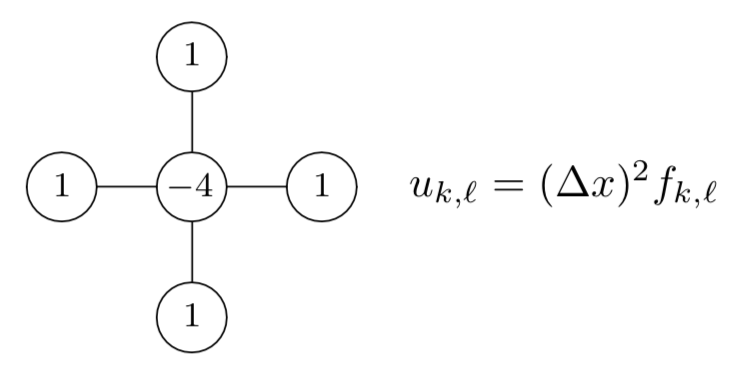
\includegraphics[width=0.4\textwidth]{five_point_stencil}
    \end{center}
    \item \bheading{solving linear equation} Main idea of finite difference method is to associate every grid point having an index in $\bI_{\Dx}^{\circ}$ a single linear equation. Solving a system of linear equations whose solution is our approximation $\bu = (u_{k,l})_{(k,l)\in \bI_{\Dx}^{\circ}}$. Performance of finite difference is evaluated with 
    \begin{enumerate}
        \item nonsingular linear system (such that $\bu$ exists and is unique)
        \item for $\Dx \to 0$, the convergence of $\bu$ to exact solution of Poisson equation and error
        \item efficient and robust ways to solve sparse linear systems
    \end{enumerate}
    \item \bheading{A simplified grid} over a square $\Omega$. Let 
    \[
        \Omega = \pc{(x,y) \mid 0 < x,y < 1}    
        \quad \quad
        \Dx = 1/(m+1)
        \quad \quad
        (x_0, y_0) = 0
    \]
    \begin{center}
        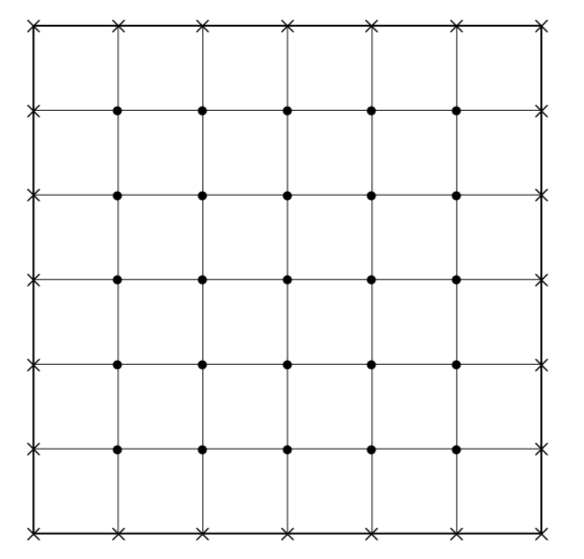
\includegraphics[width=0.3\textwidth]{simplified_grid}
    \end{center}
    \item \bheading{numerical example on Laplace equation} indicates that error decreases by a factor of 4 when number of steps $m$ increase by a factor of 2.
    \item \bheading{discretization to a system of linear equations} Rearrange $u_{k,l}$ to $\bu \in \R^s$ where $s=m^2$ according to some permutation $\pc{\p{k_i, l_i)}}_{i=1,2,\cdots,m}$ and write 
    \[
        A \bu = \bb    
    \]
    where $A$ is $s\times s$ matrix and $\bb \in\R^s$ includes both $(\Dx)^2 f_{k,l}$ and boundary values.
    \item \bheading{lemma (unique solution to linear system)} $A$ from previous is symmetric and the set of its eigenvalues is 
    \[
        \sigma(A) = \pc{
            \lambda_{\alpha,\beta} \mid \alpha,\beta = 1,2,\cdots,m
        }
    \]
    where 
    \[
        \lambda_{\alpha,\beta} = -4\pc{
            \sin^2 \pb{
                \frac{\alpha\pi}{2(m+1)}
            } + 
            \sin^2 \pb{
                \frac{\beta\pi}{2(m+1)}
            }
        }
    \]
    \begin{proof}
        Symmetry follows by examining matrix $A$. To find eigenvalues of $A$, find nonzero functions $(v_{k,l})_{k,l=0,1,\cdots,m+1}$ such that $v_{k,0} = v_{k,m+1}= v_{0,l} = v_{m+1,l} = 0$ where $k,l=1,2,\cdots, m$ such that 
        \[
            v_{k-1,l} + v_{k+1,l} + v_{k,l-1} + v_{k,l+1} - 4v_{k,l}  = \lambda v_{k,l}
            \quad 
            k,l = 1,2,\cdots, m   
        \]
        is satisfied for some $\lambda$. It follows that $(v_{k,l})$ is an eigenvector and $\lambda$ is the corresponding eignvalue of $A$. Given $\lambda_{\alpha,\beta}$ for some $\alpha,\beta$, we show that
        \[
            v_{k,l} = \sin\p{\frac{k\alpha\pi}{m+1}} \sin \p{\frac{l\beta\pi}{m+1}}
            \quad 
            k,l = 0,1,\cdots,m+1
        \]
        is the corresponding eigenvector by verifying above formula.
    \end{proof}
    \item \bheading{corollary} The matrix $A$ is negative definite and, therefore, nonsingular
    \begin{proof}
        $A$ is symmetric and from previous lemma eigenvalues are negative, therefore it is negative definite and nonsingular
    \end{proof}
    \item \bheading{eigenvalues of the Laplace operator} The function $v$, not identically zero, is said to be an \textit{eigenfunction} of $\nabla^2$ in a domain $\Omega$ and $\lambda$ is the corresponding eigenvalue if $v$ vanishes along $\partial \Omega$ and satisfies within $\Omega$ the equation $\nabla^2 v = \lambda v$. Note eigenvalues and eigenfunctions of the Laplace operator $\nabla^2$ over $(0,1)^2$ are \textit{related to} eigenvalues and eigenvectors of the matrix $A$. Given $\alpha,\beta$, eigenvalue of $\nabla^2$ and the corresponding eigenfunction is given by
    \begin{align*}
        \lambda_{\alpha,\beta} 
            &= -(\alpha^2 + \beta^2) \pi^2 \\
        v(x,y) 
            &= \sin(\alpha\pi x) \sin(\beta\pi y)
            \quad \quad 
            x,y\in [0,1]
    \end{align*}
    We can easily verify that 
    \begin{align*}
        \nabla^2 v 
        &= -\alpha^2 \pi \sin(\alpha\pi x) \sin(\beta \pi y) - \beta^2 \pi \sin(\alpha\pi x) \sin(\beta\pi y) \\
        &= -(\alpha^2 + \beta^2) \pi^2 v
    \end{align*}
    $v$ obeys boundary conditions. Note eigenvectors $v_{k,l}$ for $A$ can be obtained by sampling of the eigenfunction $v$ at grid points 
    \[
        \pc{\p{
            \frac{k}{m+1}, \frac{l}{m+1}
        }}_{k,l=0,1,\cdots,m+1}
    \]
    Note $(\Dx)^{-2} \lambda_{\alpha,\beta}$ is a good approximation to $-(\alpha^2 + \beta^2) \pi^2$ provided $\alpha,\beta$ are small in comparison with $m$. Note we can expand $\sin^2$ in a power series
    \begin{align*}
        \frac{\lambda_{\alpha,\beta}}{\p{\Dx}^2}
            =& -4 \p{
                \pc{
                    \p{\frac{\alpha\pi}{2(m+1)}}^2 - \frac{1}{3} \p{\frac{\alpha\pi}{2(m+1)}}^4 + \cdots
                } + 
                \pc{
                    \p{\frac{\beta\pi}{2(m+1)}}^2 - \frac{1}{3} \p{\frac{\beta\pi}{2(m+1)}}^4 + \cdots
                } } \\
            =& -(\alpha^2 + \beta^2) \pi^2 + \frac{1}{12} (\alpha^4 + \beta^4) \pi^4 (\Dx)^2  + \sO((\Dx)^4)
    \end{align*}
    \item \bheading{theorem (convergence)} Subject to sufficient smoothness of the function $f$ and the boundary conditions, there exists a number $c>0$, independent of $\Dx$, such that 
    \[
        \norm{\be} \leq c(\Dx)^2
        \quad \quad \Dx \to 0   
    \]
    or equivalently 
    \[
        \lim_{\Dx \to 0} \norm{\be}_{\infty} = 0
    \]
    where $\be \in \R^s$, $s=m^2$ in same order as that of $\bu$. Denote $e_{k,l} = u_{k,l} - \tilde{u}_{k,l}$ as error of the five point formula at the $(k,l)$th grid point.
    \item \bheading{handle near boundary grid points} approximate $z''$ at $P$ in $x$ direction as a linear combination of value of $z$ at $P,Q,T$. The coefficient of terms can be determined via Taylor expansion of $z_{x_0-\Dx},z_{x_0},z_{x_0+\tau\Dx}$ at $a=x_0$ and solve a $3\times 3$ linear system. The error of approximation is $\sO(\Dx)$
    \begin{align*}
        \frac{1}{(\Dx)^2} &\pb{
            \frac{2}{\tau+1} z(x_0-\Dx) - \frac{2}{\tau} z(x_0) + \frac{2}{\tau(\tau+1)} z(x_0+\tau\Dx)
        } \\
        &= z''(x_0) + \frac{1}{3} (\tau-1)z'''(x_0)\Dx + \sO((\Dx)^2)
    \end{align*}
    To achieve $\sO((\Dx)^2)$ order for the error, we use value of $z$ at 4 grid points $V,Q,P,T$ to approximate $z''$. Coefficient to linear term can be determined with Taylor expansion and solve a $4\times 4$ linear system.
    \begin{align*}
        \frac{1}{(\Dx)^2} &\pb{
            \frac{\tau-1}{\tau+2} z(x_0-2\Dx) + \frac{2(2-\tau)}{\tau+1} z(x_0-\Dx) - \frac{3-\tau}{\tau} z(x_0) + \frac{6}{\tau(\tau+1)(\tau+2)} z(x_0+\tau\Dx)
        } \\ 
        &= z''(x_0) + \sO((\Dx)^2)
    \end{align*}
    In total, a good approximation to $\nabla^2 u$ at $P$ requires 6 points. For $P$ corresponding to grid $(k,l)$, we obtain the following linear equation for constructing $A$ and $b$ for both first order and second order approximations
    \[
        \frac{2}{\tau+1} u_{k-1,l} + \frac{2}{\tau(\tau+1)} u_{k+\tau,l} + u_{k,l-1} + u_{k, l+1} - \frac{2+2\tau}{\tau} u_{k,l} = (\Dx)^2 f_{k,l}
    \]
    \[
        \frac{\tau-1}{\tau+2} u_{k-2,l} + \frac{2(2-\tau)}{\tau+1} u_{k-1,l} + \frac{6}{\tau(\tau+1)(\tau+2)} u_{k+\tau, l} + u_{k,l-1} + u_{k,l+1} - \frac{3+\tau}{\tau} u_{k,l}
        = (\Dx)^2 f_{k,l}
    \]
    \begin{center}
        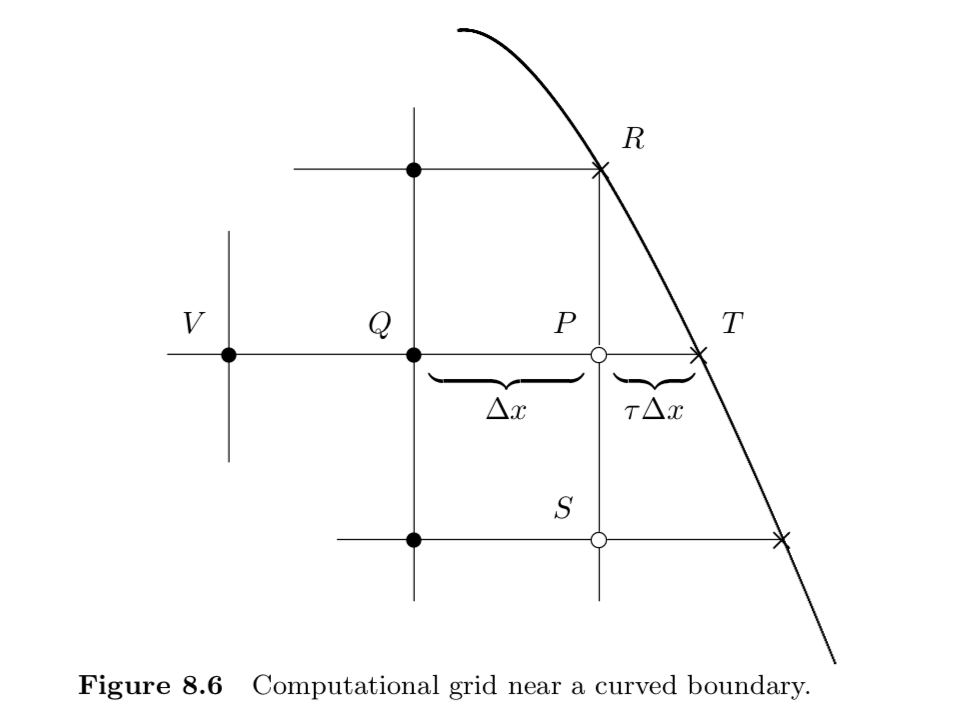
\includegraphics[width=4in]{near_boundary_stencil}
    \end{center}
\end{enumerate}


\end{document}